%%%%%%%%%%%%%%%%%%%%%%%%%%%%%%%%%%%%%%%%%%%%%%%%%%%%%%%%%%%%%%%
%% OXFORD THESIS TEMPLATE

% Use this template to produce a standard thesis that meets the Oxford University requirements for DPhil submission
%
% Originally by Keith A. Gillow (gillow@maths.ox.ac.uk), 1997
% Modified by Sam Evans (sam@samuelevansresearch.org), 2007
% Modified by John McManigle (john@oxfordechoes.com), 2015
% Modified by Ulrik Lyngs (ulrik.lyngs@cs.ox.ac.uk), 2018-, for use with R Markdown
%
% Ulrik Lyngs, 25 Nov 2018: Following John McManigle, broad permissions are granted to use, modify, and distribute this software
% as specified in the MIT License included in this distribution's LICENSE file.
%
% John commented this file extensively, so read through to see how to use the various options.  Remember that in LaTeX,
% any line starting with a % is NOT executed.

%%%%% PAGE LAYOUT
% The most common choices should be below.  You can also do other things, like replace "a4paper" with "letterpaper", etc.

% 'twoside' formats for two-sided binding (ie left and right pages have mirror margins; blank pages inserted where needed):
%\documentclass[a4paper,twoside]{templates/ociamthesis}
% Specifying nothing formats for one-sided binding (ie left margin > right margin; no extra blank pages):
%\documentclass[a4paper]{ociamthesis}
% 'nobind' formats for PDF output (ie equal margins, no extra blank pages):
%\documentclass[a4paper,nobind]{templates/ociamthesis}

% As you can see from the line below, oxforddown uses the a4paper size, 
% and passes in the binding option from the YAML header in index.Rmd:
\documentclass[a4paper, nobind]{templates/ociamthesis}


%%%%% ADDING LATEX PACKAGES
% add hyperref package with options from YAML %
\usepackage[pdfpagelabels]{hyperref}
% handle long urls
\usepackage{xurl}
% change the default coloring of links to something sensible
\usepackage{xcolor}

\definecolor{mylinkcolor}{RGB}{0,0,139}
\definecolor{myurlcolor}{RGB}{0,0,139}
\definecolor{mycitecolor}{RGB}{0,33,71}

\hypersetup{
  hidelinks,
  colorlinks,
  linktocpage=true,
  linkcolor=mylinkcolor,
  urlcolor=myurlcolor,
  citecolor=mycitecolor
}


% add float package to allow manual control of figure positioning %
\usepackage{float}

% enable strikethrough
\usepackage[normalem]{ulem}

% use soul package for correction highlighting
\usepackage{color, soulutf8}
\definecolor{correctioncolor}{HTML}{CCCCFF}
\sethlcolor{correctioncolor}
\newcommand{\ctext}[3][RGB]{%
  \begingroup
  \definecolor{hlcolor}{#1}{#2}\sethlcolor{hlcolor}%
  \hl{#3}%
  \endgroup
}
% stop soul from freaking out when it sees citation commands
\soulregister\ref7
\soulregister\cite7
\soulregister\citet7
\soulregister\autocite7
\soulregister\textcite7
\soulregister\pageref7

%%%%% FIXING / ADDING THINGS THAT'S SPECIAL TO R MARKDOWN'S USE OF LATEX TEMPLATES
% pandoc puts lists in 'tightlist' command when no space between bullet points in Rmd file,
% so we add this command to the template
\providecommand{\tightlist}{%
  \setlength{\itemsep}{0pt}\setlength{\parskip}{0pt}}
 
% allow us to include code blocks in shaded environments

% User-included things with header_includes or in_header will appear here
% kableExtra packages will appear here if you use library(kableExtra)
\usepackage{booktabs}
\usepackage{longtable}
\usepackage{array}
\usepackage{multirow}
\usepackage{wrapfig}
\usepackage{float}
\usepackage{colortbl}
\usepackage{pdflscape}
\usepackage{tabu}
\usepackage{threeparttable}
\usepackage{threeparttablex}
\usepackage[normalem]{ulem}
\usepackage{makecell}
\usepackage{xcolor}


%UL set section header spacing
\usepackage{titlesec}
% 
\titlespacing\subsubsection{0pt}{24pt plus 4pt minus 2pt}{0pt plus 2pt minus 2pt}


%UL set whitespace around verbatim environments
\usepackage{etoolbox}
\makeatletter
\preto{\@verbatim}{\topsep=0pt \partopsep=0pt }
\makeatother


%%%%%%% PAGE HEADERS AND FOOTERS %%%%%%%%%
\usepackage{fancyhdr}
\setlength{\headheight}{15pt}
\fancyhf{} % clear the header and footers
\pagestyle{fancy}
\renewcommand{\chaptermark}[1]{\markboth{\thechapter. #1}{\thechapter. #1}}
\renewcommand{\sectionmark}[1]{\markright{\thesection. #1}} 
\renewcommand{\headrulewidth}{0pt}





% UL page number position 
\fancyfoot[C]{\emph{\thepage}} %regular pages
\fancypagestyle{plain}{\fancyhf{}\fancyfoot[C]{\emph{\thepage}}} %chapter pages




%%%%% SELECT YOUR DRAFT OPTIONS
% This adds a "DRAFT" footer to every normal page.  (The first page of each chapter is not a "normal" page.)

% IP feb 2021: option to include line numbers in PDF

% for line wrapping in code blocks
\usepackage{fancyvrb}
\usepackage{fvextra}
\DefineVerbatimEnvironment{Highlighting}{Verbatim}{breaklines=true, breakanywhere=true, commandchars=\\\{\}}

% This highlights (in blue) corrections marked with (for words) \mccorrect{blah} or (for whole
% paragraphs) \begin{mccorrection} . . . \end{mccorrection}.  This can be useful for sending a PDF of
% your corrected thesis to your examiners for review.  Turn it off, and the blue disappears.


%%%%% BIBLIOGRAPHY SETUP
% Note that your bibliography will require some tweaking depending on your department, preferred format, etc.
% If you've not used LaTeX before, I recommend just using pandoc for citations -- this is what's used unless you specific e.g. "citation_package: natbib" in index.Rmd
% If you're already a LaTeX pro and are used to natbib or something, modify as necessary.

% this allows the latex template to handle pandoc citations




% Uncomment this if you want equation numbers per section (2.3.12), instead of per chapter (2.18):
%\numberwithin{equation}{subsection}


%%%%% THESIS / TITLE PAGE INFORMATION
% Everybody needs to complete the following:




% Master's candidates who require the alternate title page (with candidate number and word count)
% must also un-comment and complete the following three lines:

% Uncomment the following line if your degree also includes exams (eg most masters):
%\renewcommand{\submittedtext}{Submitted in partial completion of the}
% Your full degree name.  (But remember that DPhils aren't "in" anything.  They're just DPhils.)


% Term and year of submission, or date if your board requires (eg most masters)



%%%%% YOUR OWN PERSONAL MACROS
% This is a good place to dump your own LaTeX macros as they come up.

% To make text superscripts shortcuts
\renewcommand{\th}{\textsuperscript{th}} % ex: I won 4\th place
\newcommand{\nd}{\textsuperscript{nd}}
\renewcommand{\st}{\textsuperscript{st}}
\newcommand{\rd}{\textsuperscript{rd}}

%%%%% THE ACTUAL DOCUMENT STARTS HERE
\begin{document}

%%%%% CHOOSE YOUR LINE SPACING HERE
% This is the official option.  Use it for your submission copy and library copy:
\setlength{\textbaselineskip}{22pt plus2pt}
% This is closer spacing (about 1.5-spaced) that you might prefer for your personal copies:
%\setlength{\textbaselineskip}{18pt plus2pt minus1pt}

% You can set the spacing here for the roman-numbered pages (acknowledgements, table of contents, etc.)
\setlength{\frontmatterbaselineskip}{17pt plus1pt minus1pt}

% UL: You can set the line and paragraph spacing here for the separate abstract page to be handed in to Examination schools
\setlength{\abstractseparatelineskip}{13pt plus1pt minus1pt}
\setlength{\abstractseparateparskip}{0pt plus 1pt}

% UL: You can set the general paragraph spacing here - I've set it to 2pt (was 0) so
% it's less claustrophobic
\setlength{\parskip}{2pt plus 1pt}

%
% Customise title page
%
\def\crest{}
\renewcommand{\university}{}
\renewcommand{\submittedtext}{}
\renewcommand{\thesistitlesize}{\fontsize{22pt}{28pt}\selectfont}
\renewcommand{\gapbeforecrest}{25mm}
\renewcommand{\gapaftercrest}{25mm
}


% Leave this line alone; it gets things started for the real document.
\setlength{\baselineskip}{\textbaselineskip}


%%%%% CHOOSE YOUR SECTION NUMBERING DEPTH HERE
% You have two choices.  First, how far down are sections numbered?  (Below that, they're named but
% don't get numbers.)  Second, what level of section appears in the table of contents?  These don't have
% to match: you can have numbered sections that don't show up in the ToC, or unnumbered sections that
% do.  Throughout, 0 = chapter; 1 = section; 2 = subsection; 3 = subsubsection, 4 = paragraph...

% The level that gets a number:
\setcounter{secnumdepth}{2}
% The level that shows up in the ToC:
\setcounter{tocdepth}{1}


%%%%% ABSTRACT SEPARATE
% This is used to create the separate, one-page abstract that you are required to hand into the Exam
% Schools.  You can comment it out to generate a PDF for printing or whatnot.

% JEM: Pages are roman numbered from here, though page numbers are invisible until ToC.  This is in
% keeping with most typesetting conventions.
\begin{romanpages}

% Title page is created here

%%%%% DEDICATION

%%%%% ACKNOWLEDGEMENTS


%%%%% ABSTRACT


%%%%% MINI TABLES
% This lays the groundwork for per-chapter, mini tables of contents.  Comment the following line
% (and remove \minitoc from the chapter files) if you don't want this.  Un-comment either of the
% next two lines if you want a per-chapter list of figures or tables.
\dominitoc % include a mini table of contents

% This aligns the bottom of the text of each page.  It generally makes things look better.
\flushbottom

% This is where the whole-document ToC appears:


% Uncomment to generate a list of tables:
%%%%% LIST OF ABBREVIATIONS
% This example includes a list of abbreviations.  Look at text/abbreviations.tex to see how that file is
% formatted.  The template can handle any kind of list though, so this might be a good place for a
% glossary, etc.

% The Roman pages, like the Roman Empire, must come to its inevitable close.
\end{romanpages}

%%%%% CHAPTERS
% Add or remove any chapters you'd like here, by file name (excluding '.tex'):
\flushbottom

% all your chapters and appendices will appear here
\hypertarget{rmd-basics}{%
\chapter{Results}\label{rmd-basics}}

\minitoc 

\noindent

\hypertarget{learner-characteristics}{%
\section{Learner Characteristics}\label{learner-characteristics}}

When asked the amount of time participants have used a chatbot- in any form or subject: 23 stated they had never used a chatbot, educational or not. Further, 18/42 having used a chatbot at least once for between 0-4 hours of use in total. Two individuals had spent much longer time with usage- these were a learning technologist associated with the CEPEH team, and a mature student.
In short, this sample of participants did not regularly use chatbots for their course learning, but 1/3 had used one in some form previously.

Most learners use books or online books as resources. They may use multiple sources however they were asked to note
the primary source. Only 6 stated their primary sources were \emph{Online videos/interactive materials} which includes
such tools as chatbots.

The first boxplot (\ref{fig:Boxplotsplits2}) shows learners perceptions of easy of use of mobile app and other educational mobile resources

\begin{figure}
\centering
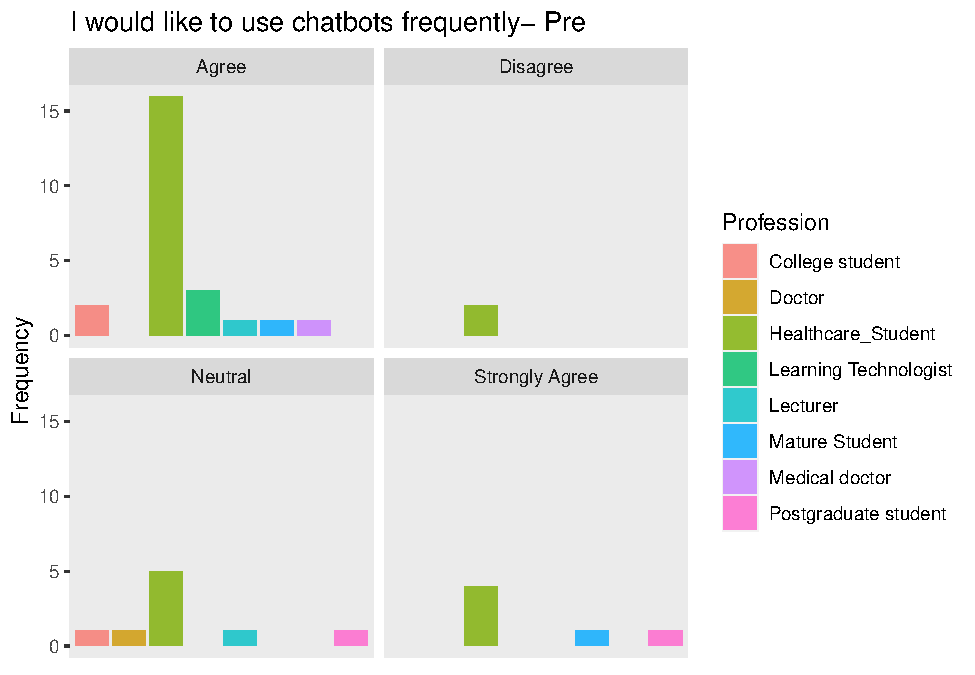
\includegraphics{02-Results_files/figure-latex/Boxplotsplits2-1.pdf}
\caption{\label{fig:Boxplotsplits2}Usage Freq Pre.}
\end{figure}

\begin{longtable}[]{@{}lr@{}}
\toprule()
Previous\_Chatbot\_Usage & n \\
\midrule()
\endhead
1-4 hours & 15 \\
10-19 hours & 1 \\
20+ hours & 1 \\
5-9 hours & 2 \\
Never & 23 \\
\bottomrule()
\end{longtable}

\#\#Post-Intervention Results and Comparision

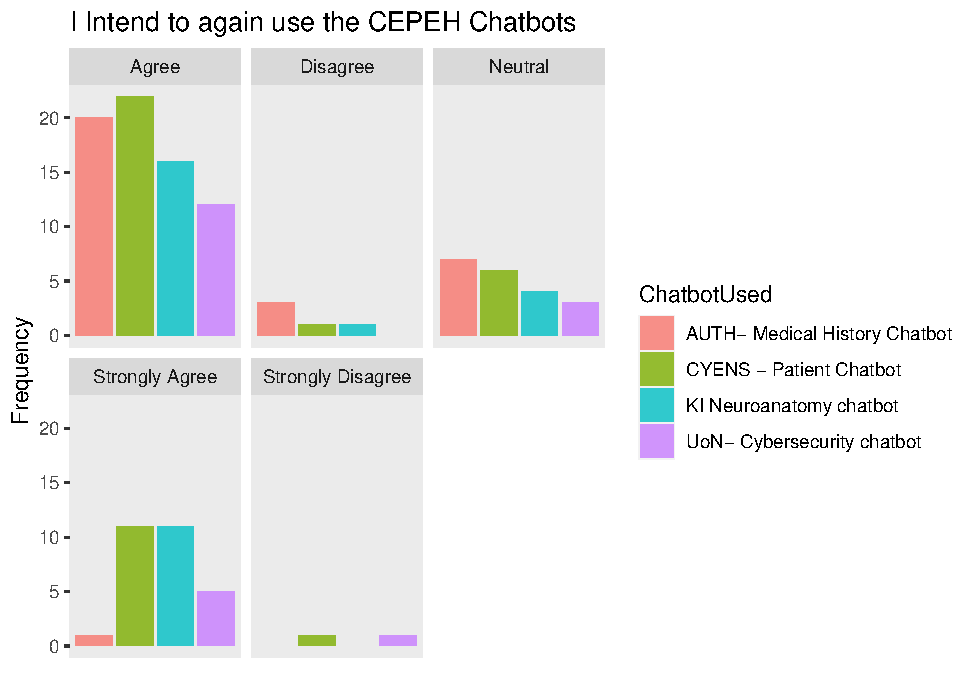
\includegraphics{02-Results_files/figure-latex/Boxplotsplits4-1.pdf}
For CYENS, even though the knowledge of the topic was not perceived to improve by some participants, this box plot shows how 34/42 stated they would reuse the chatbot developed by CYENS.

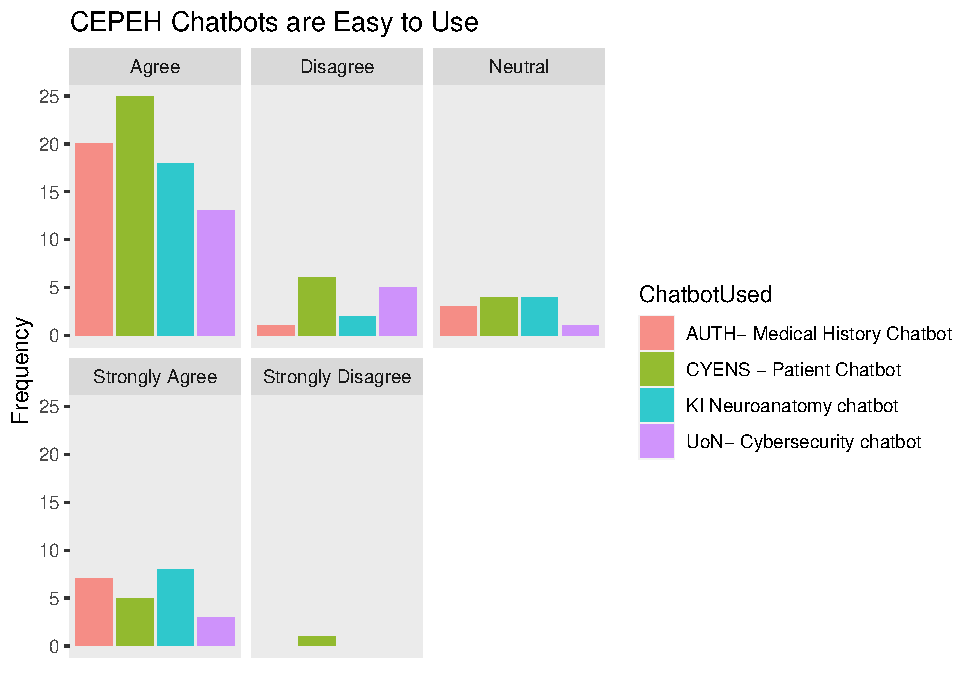
\includegraphics{02-Results_files/figure-latex/Boxplotsplits3-1.pdf}
There was only 1 `Strongly Disagree' response.
The agreement options counted for the majority of the data.

\hypertarget{other-findings}{%
\subsection{Other Findings}\label{other-findings}}

Other questions

I intend to continue using chatbots in the future (BI1)
The chatbot provided the information I needed with minimal commands
My knowledge of the topic improved after i had used the Chatbot
My confidence in understanding the topic improved after I had used the
Chatbot
The chatbot provided me with the type of response i expected from asking
a tutor/lecturer
The information provided was reliable
The chatbot has a high level of trustworthiness
The duration of conversations to find my answer was too long
The videos/images provided were useful to my questions
The chatbot exceeded my expectation of how it could help me
The chatbot exceeded my expectation of how it could engage with me
I think this learning method could help me to acquire knowledge
I would use this tool again as it has some value to me
I think i will actively use this learning method
I believe I had some choice about learning during chatbot use
I would trust the chatbot to provide me with information for my course
One piece of knowledge i learned from the chatbot was..

Repeated Measures t-test, aka paired t-test (before and after measurements)

This t-test compares confident using mobile chatbots before and after CEPEH chatbot usage.

\hypertarget{system-usability-scale-sus-scores}{%
\subsection{System Usability Scale (SUS) Scores}\label{system-usability-scale-sus-scores}}

\emph{Note= The amount of `agreement' is defined as the addition of `Agree'
and `Strongly agree' responses.}

The SUS score should consist of 10 items. However, some SUS questions
were improved upon by 1 or more CUQ questions, specifically to this
Chatbot study. The SUS results would be overshadowed by the CUQ scores,
expect 2 that did not have cross-over. The two questions were:

\begin{itemize}
\tightlist
\item
  I would like to use the CEPEH chatbot I tested, more frequently
  (SUS1)(post)
\item
  I felt confident using the CEPEH chatbot (SUS2)(post)
\end{itemize}

This meant the score of the SUS was not created, however the CUQ score
better represented the Learners' perceptions of the CEPEH chatbot in
terms of feasibility of reuse and acceptability in healthcare curricula.

\begin{longtable}[]{@{}llr@{}}
\toprule()
Keep\_Using\_Chatbots & Confident & Count \\
\midrule()
\endhead
Agree & Agree & 44 \\
Agree & Disagree & 5 \\
Agree & Neutral & 11 \\
Agree & Strongly Agree & 6 \\
Disagree & Agree & 6 \\
Disagree & Disagree & 5 \\
Disagree & Neutral & 4 \\
Neutral & Agree & 10 \\
Neutral & Disagree & 1 \\
Neutral & Neutral & 6 \\
Not Applicable & Not Applicable & 3 \\
Strongly Agree & Agree & 10 \\
Strongly Agree & Not Applicable & 1 \\
Strongly Agree & Strongly Agree & 12 \\
Strongly Disagree & Agree & 1 \\
Strongly Disagree & Strongly Agree & 1 \\
\bottomrule()
\end{longtable}

\hypertarget{technology-acceptance-model}{%
\subsection{Technology Acceptance Model}\label{technology-acceptance-model}}

The TAM had 3 sections (Ease of Use, Perceived Usefulness, and Intention
of Use). Ease of Use results showed significant increases in Users'
usage with each Chatbot. Perceived Usefulness: There were not
significant findings for the Perceived usefulness. The justification for
this may be due to being early versions of applications with limited
functionality and functions which can be difficult for user to
experience the intended further range of features and learning
exercises.

Intention of Use: For users' intentions to use within their course, the
result of the Mann-Whitney U test was not significant, U = , z = , p = .
in their intentions before use (m=xx, mode=xx) compared to after (m=xx,
mode=x), however there was improvement therefore the chatbots may have
more benefit than expected by students.

\hypertarget{chatbot-usabilty-questionanire-cuq}{%
\section{Chatbot Usabilty Questionanire (CUQ)}\label{chatbot-usabilty-questionanire-cuq}}

\hypertarget{cuq-calcuation-tool}{%
\subsection{CUQ Calcuation tool}\label{cuq-calcuation-tool}}

The CUQ was developed by researchers at Ulster University,\href{\%3Ca\%20href=\%22https://www.ulster.ac.uk/research/topic/computer-science/artificial-intelligence/projects/cuq\%22}{Link}
and as the calculation can be complex a dedicated calculation tool has been created.
Please download the CEPEH CUQ calculation tool which has all of the data entered, so you can see the CEPEH CUQ scoring.

\href{CUQ-Calculation-Tool.xlsx}{click here to download CUQ calc tool}

\href{cuq.png}{click here to download CUQ score image}
*mobile download disabled

\begin{figure}

{\centering 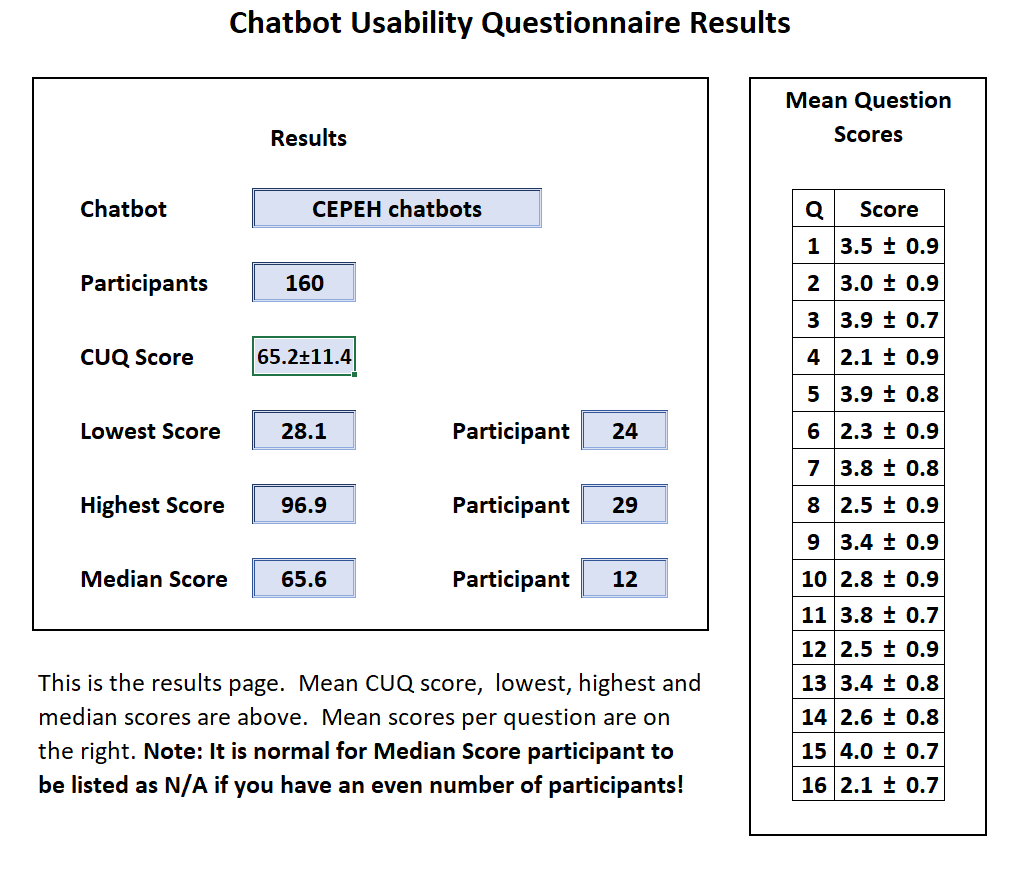
\includegraphics[width=0.75\linewidth]{cuq} 

}

\caption{A marvel-lous meme}(\#fig:cuq image)
\end{figure}

The score for all 3 chatbots grouped was 65.2/100,
This scoring system was designed to be comparable to SUS and may be
freely used alongside it, or in combination with other usability
metrics. There has been evidence of correlation of 76\% between the CUQ
and SUS therefore we expect the SUS scored to be between 48.75 and 81\%.
We believe the CUQ has more validity towards measuring the concepts of
interest on this study.

\href{\%3Ca\%20href=\%22https://dl.acm.org/doi/pdf/10.1145/3335082.3335094?casa_token=rGs2gNvKuLkAAAAA:Cd8Qn3QywYHZGYJzbD5CU1dVFWHPLGzDnmQYue6ix-AcqOkWLa7VN4GuzvfrZR2DhhvEAoZOF_2T}{Read the CUQ development paper, see page 3 for correlation}

Figure shows the CUQ scores as a box plot to highlight the range of Usability of the resources. Further exploration is required to understand which elements are causing this spread.

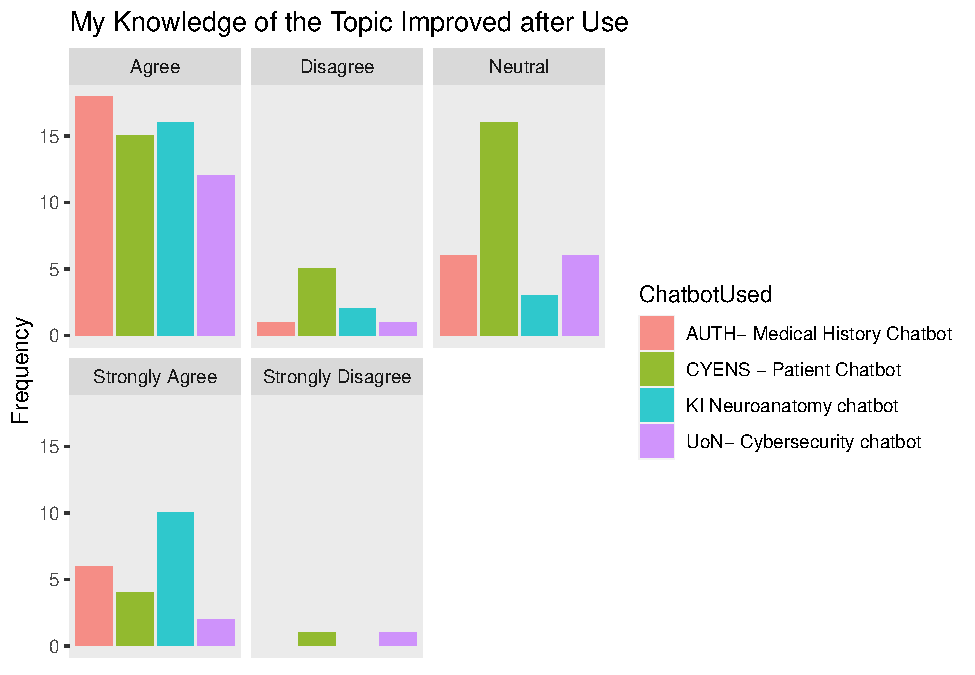
\includegraphics{02-Results_files/figure-latex/Boxplotsplits5-1.pdf}
CYENS chatbot had around 10 more participants stating that they were neutral on gaining knowledge of the topic

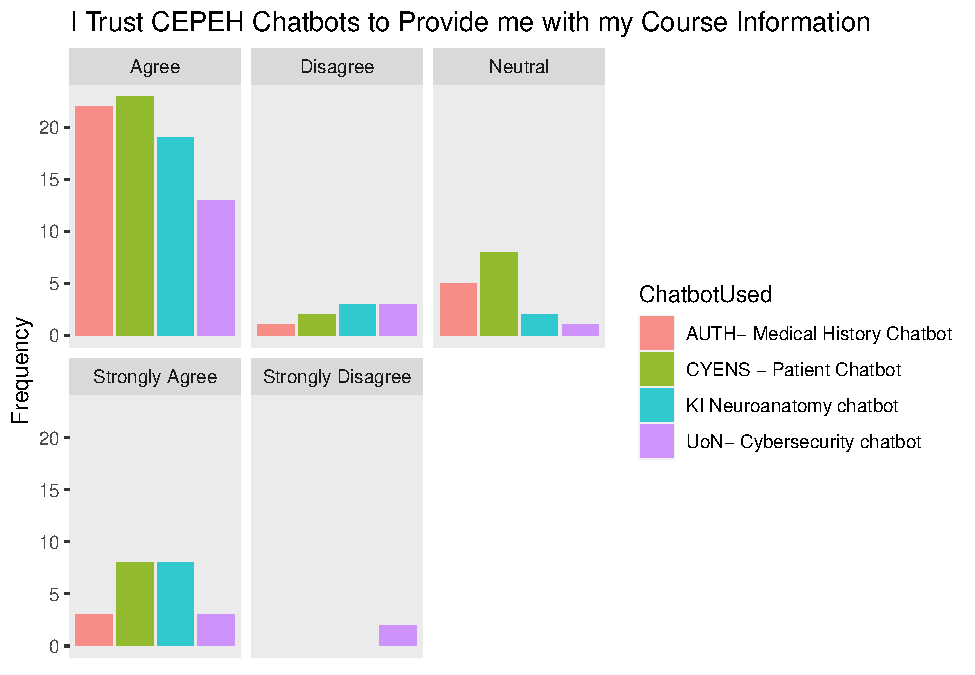
\includegraphics{02-Results_files/figure-latex/Boxplotsplits6-1.pdf}

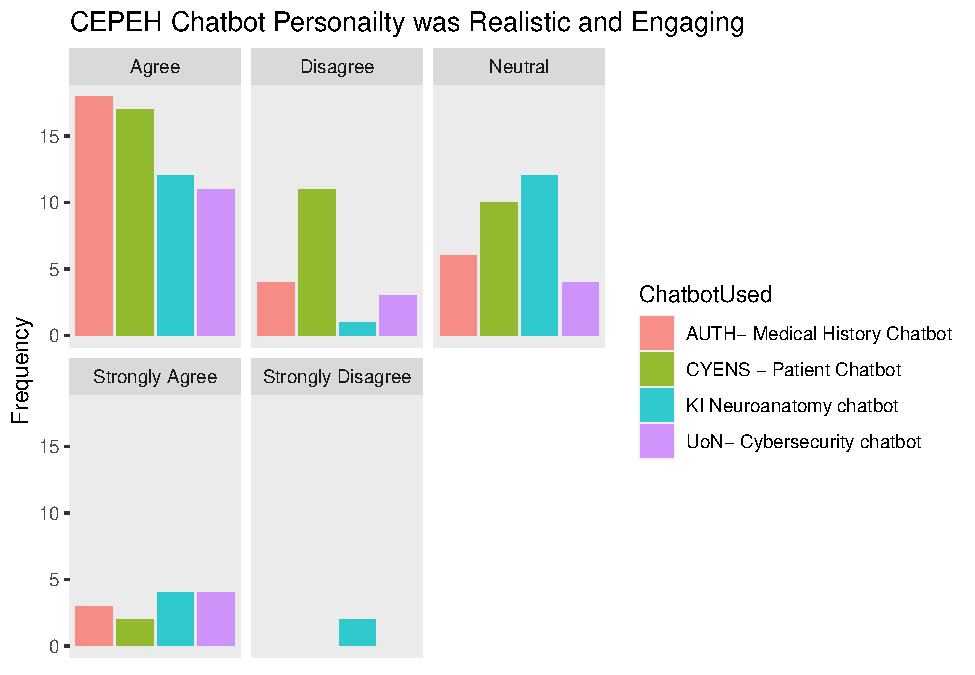
\includegraphics{02-Results_files/figure-latex/Boxplotsplits7-1.pdf}
There was mixed results for the chatbot used being realistic and engaging. This question has two descriptive terms however based on the other results we understand that the chatbots' NLP logic, or ability to respond required improvement to be more `smooth' in replying. The primary limitation was found in the `robotic' interactions(See Figure 10). This was investigated further in the `Text Mining' and `Sentiment Analysis' sections.

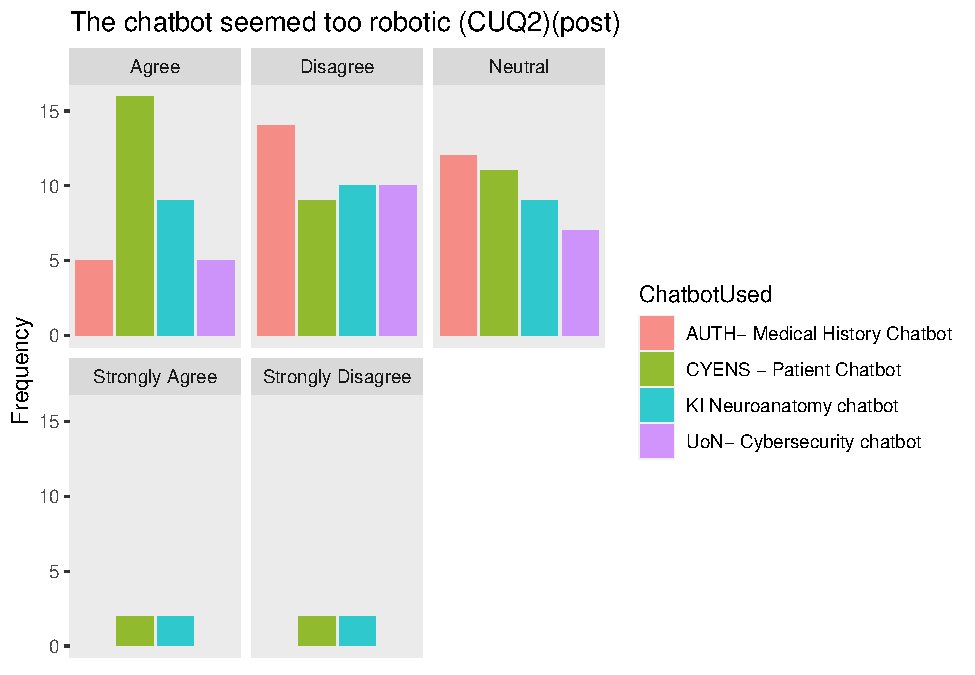
\includegraphics{02-Results_files/figure-latex/Boxplotsplits8-1.pdf}

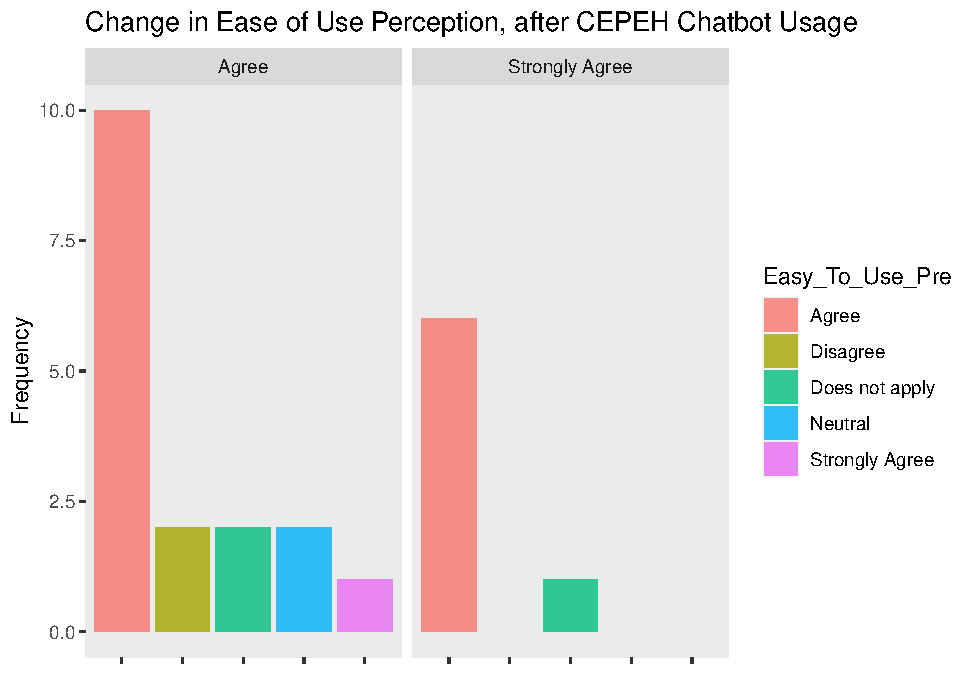
\includegraphics{02-Results_files/figure-latex/Boxplotsplits9-1.pdf}

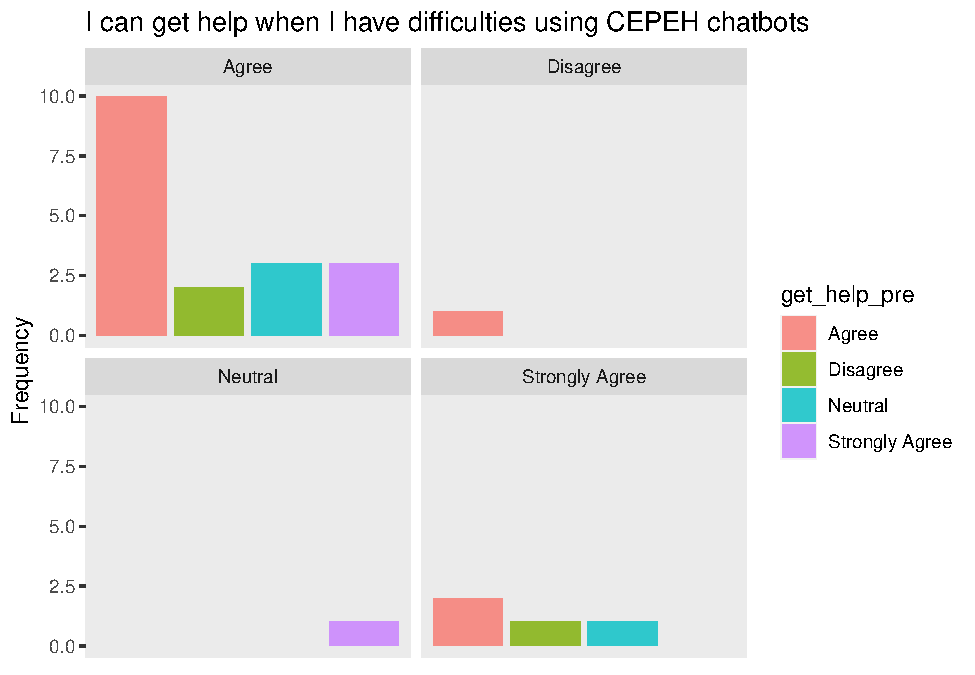
\includegraphics{02-Results_files/figure-latex/Boxplotsplits10-1.pdf}
Those who disagreed or were neutral in the pre usage measure, improved their understanding that help was available
with the CEPEH chatbots. After usage, 40 participants agreed they could get help if they had difficulty using the
resources.

\hypertarget{inferential-statistics}{%
\section{Inferential Statistics}\label{inferential-statistics}}

%%%%% REFERENCES


\end{document}
